%A per-group write-up of 5–9 polished pages (due on the last day of class). The write-up should include (1) a technical description of the team’s solution, including how the team has ensured the solution is correct, (2) a brief comparison of the solution with other similar software for related problems (if any).

\documentclass[12pt,letterpaper]{report}
\usepackage[utf8]{inputenc}
\usepackage{amsmath}
\usepackage{amsfonts}
\usepackage{amssymb}
\usepackage{graphicx}
\usepackage[left=1in,right=1in,top=1in,bottom=1in]{geometry}
\usepackage{rotating}
\usepackage{hyperref}
\usepackage{natbib}
\bibliographystyle{abbrvnat}
\setcitestyle{authoryear,open={(},close={)}}
\begin{document}
\begin{center}
{\huge \textbf{Final Report}}\\
Charlotte Darby, Yue Lu, Tony Tong\\
\{cdarby, yuel2, xtong\} @andrew.cmu.edu\\
Bioinformatics Data Integration Practicum 2016\\
\end{center}

{\Large\textbf{Solution summary}}\\

The bioinformatics pipeline we developed for our project is designed to predict transcription termination sites (TTS) in \textsl{Zea mays}. First, the user chooses a set of known TTS as the pattern. Then, our pipeline employs motif discovery using MEME (Multiple EM for Motif Elicitation) \cite{meme} and the random forest algorithm for machine learning \cite{rf} to characterize the pattern. Once the pattern has been learned, the model can be used to predict new TTS in the maize genome.\\

\indent For this context, we define a ``known TTS'' as the final base pair of a cDNA sequence in the maize AGPv3 genome build. To build a pattern, we characterize the patterns in the 300bp upstream and 100bp downstream of the end of a TTS. \\

{\Large\textbf{Related work}}\\

\indent SignalSleuth \citep{loke05} characterizes poly-A sites in \textsl{Arabidopsis thaliana} using a brute-force enumeration of patterns found in regions surrounding known sites. Using this tool, the authors discovered characteristic motifs, base pair composition patterns, and secondary structure elements around poly-A sites.\\

\indent The PASS software presented in \citep{ji07} uses a generalized hidden Markov model (GHMM) to identify poly-A sites in \textsl{Arabidopsis}. An advantage of using a GHMM is that it can characterize motifs that are not easily represented in a PSSM; for example, those including indels or that can appear in multiple copies. They found that near upstream motifs were 6nt long, and far upstream motifs were 8nt long.\\

\indent \citet{shen08} used 300bp upstream and 100bp downstream from known TTS to characterize poly-A sites in rice, which was the reason we chose this particular window. The model of poly-A sites in Shen et al.~also used a GHMM.\\

{\Large\textbf{Data acquisition}}\\

First, we considered characterizing patterns in all cDNA sequences available from the maize AGPv3 genome build. However, there are 63235 such sequences in the complete cDNA dataset available from Ensembl. MEME cannot handle an input dataset of this size. Indeed, it is unlikely that a significant motif (that is not just a characteristic of the underlying sequence AT/GC composition) would be detected in the whole dataset, even in MEME’s zero-or-one-per-sequence mode. If there are important motifs in a certain segment that can be characterized by a PSSM, they may not occur in enough genes in the dataset to be detected in this way.\\

\indent Instead, we pared down the cDNA dataset. One way to filter genes from the dataset is to search by Gene Ontology (GO) terms \cite{go}. The Gene Ontology Consortium uses a hierarchical vocabulary to systematically annotate gene subcellular localization, biochemical process, and molecular function in selected organisms, including maize. If two genes share GO terms, this implies they have some level of shared function. Furthermore, shared GO terms may be indicative of shared regulation, especially if the function may involve differential expression under certain conditions. For example, responses to environmental conditions or cellular processes may be co-regulated. Alternative TTS may need to be activated under these conditions. To this end, particular TTS motifs may be enriched in genes with shared GO terms. We use this hypothesis to justify selecting genes with shared GO terms as the input to our pipeline. \\

\indent Our method of pattern characterization with MEME and random forests is computationally feasible on sets of about 200-600 termination sites. More are possible, if you are patient: MEME is the rate-limiting step, as it is run sequentially on all eight segments and the parallelized version is not utilized. We downloaded datasets to develop and test our model using BioMart, a feature of the Gramene/Ensembl database \cite{biomart}. BioMart appears to be quite user-friendly, and given the detailed instructions in our manual, we expect that users of the pipeline will be able to download sequences of their choice in the proper format. This step is not automated, although entering the desired GO term to our program and interacting with BioMart servers from within our program would be a nice functionality. As example datasets, we chose ``response to salt stress,'' (575 sequences) ``photosynthesis,'' (401 sequences) ``response to water deprivation,'' (250 sequences) and ``ribosome'' (247 sequences).\\

{\Large\textbf{Environment setup}}\\

We received feedback that the amount of setup work needed to run our pipeline is somewhat inconvenient. MEME 4.11.1 and Python 2.7 must be installed, and MEME will compile locally and run extensive tests to ensure all dependencies are present and updated. The Python packages used are pandas, pickle, Bio, numpy, and sklearn; some of these must be installed separately atop standard Python distributions. \\

\indent One strategy that would reduce setup time is to write the routines in Java, for example, and provide a complete .jar (or a comparable packaged runnable unit in another programming language) containing all the dependencies the program relies on. Additionally, it may be possible to include a precompiled MEME distribution with our pipeline code, or interface with the web server provided at \url{http://meme-suite.org/tools/meme}.\\

{\Large\textbf{Feature calculation}}\\

Our main strategy in feature calculation is to divide the 400bp string surrounding the known TTS into eight 50bp segments; i.e. (1-50), (51-100), and so on. It is reasonable to suppose that there may be different motifs characterizing the regions around the TTS that have a spatial arrangement. One motif may occur before the TTS, while another may occur after the TTS. We chose a 50bp segment size to balance resolution of the prediction and motif detection. With a smaller window size, we would gain higher resolution in TTS prediction. However, feature calculation and genome scanning would be more computationally intensive. Additionally, using longer segments increases the chance that a motif will be contained in that window in many sequences. Using 15bp, for example, would increase the prediction's resolution but require that a motif characterizing the region after a TTS be within (300-315) in many sequences. This is too restrictive to be biologically reasonable.\\

\indent Our 50bp window will allow us to examine the near upstream element (NUE), if it exists in maize like it does in \textsl{Arabidopsis}. In \textsl{Arabidopsis},  ``the NUE region is A rich and spans about 6 to 10 nt located between 13 and 30 nt upstream of the CS [cleavage site]'' \cite{loke05} Shen et al. (2008) found that in rice (\textsl{Oryza sativa}), the NUE generally occurs between -35 and -10. The far upstream element (FUE) may occur from -150 to -35, which actually places it in 2-3 of our segments.\\

\indent The sequences downloaded in FASTA format from Biomart are split into segments using a simple Python script, called from the \texttt{splitsegments.sh} shell script. At this step, the user chooses a short name for the dataset related to the GO term. The program is modular, so segment splitting, feature calculation and classifier building, and genome scanning are invoked separately by the user. If the user chooses to scan part of the genome and later wants to scan a different part, the classifier for this particular GO term dataset does not need to be rebuilt and MEME does not run again.\\

\indent Once the segments are split, MEME is run on all sequences for each segment; i.e. (1-50) for all sequences, then (51-100) for all sequences, and so on. The shell script \texttt{main.sh} creates directories and runs MEME on each of the segments sequentially. In the parameters, we limit the motif width to 12. With this restriction, MEME explores PSSMs of size 8, 10, and 12 according to its algorithm. Motif width is currently not a user-specified parameter, but it could be in the future. We also run MEME in only-one-per-sequence mode. For speed, and because our dataset is small, this option is reasonable. From the documentation, in this mode, ``MEME assumes that each sequence in the dataset contains exactly one occurrence of each motif. This option is the fastest and most sensitive but the motifs returned by MEME will be `blurry' (less specific) if they do not occur in every input sequence.'' \cite{meme} Another possibility would be to use zero-or-one-per-sequence mode. Here, motifs are assumed to occur at most once per sequence. However, this mode takes at least twice as long to run, according to the documentation. \\

\indent 4 motifs are returned for each segment, per another argument to the program. Number of motifs is cannot be specified by the user at this time, but it would be possible to incorporate. Motifs are returned in order of decreasing significance, and given 8 segments, this comprises 32 motif features. We think 4 is a reasonable number of motifs to use to reach a compromise between the decreased significance of later motifs and having enough features to build a good classifier. The PSSMs are parsed out of the MEME output files using a Python script. We use the log-odds representation to avoid underflow in downstream computation. We also calculate the GC content of each segment to give 40 features in total per 400bp sequence. \\

{\Large\textbf{Classification}}\\

The classifier classifies an input 400bp sequence as either ``has TTS at position 300'' or ``does not have TTS at position 300.'' We employ a random forest machine learning classifier \cite{rf} as implemented in the scikit-learn package for Python, version 0.17.0 \cite{scikit-learn}. Random forests are an ensemble method, meaning that many separate classifiers are aggregated to inform the final prediction. The individual classifiers are decision trees. A decision tree classifier creates a tree structure where every junction splits into two branches depending on the value of one particular feature. Figure \ref{fig:dtree} shows an example decision tree that classifies examples into 6 classes (capital letters at leaves) based on values of two features (X1 and X2). To classify a new example, start at the root and take the path corresponding to the properties of X1 and X2 in the new example. When a leaf is reached, assign that class to a new example. Note that features may be reused and classes may appear at more than one leaf. \\

\indent The decision at each junction is made based on the training data. A criterion, usually a type of entropy, is used to find the feature (e.g. X1) and threshold (e.g. X1 $<$ 5) that is most informative given the training examples at this junction. If the depth of a decision tree is unbounded, it can perfectly classify every unique training example. However, this is almost certainly overfitting. To combat this, the tree can be given a maximum depth (maximum number of decision junctions between a leaf and the top-most junction). Now the leaves may have training examples of different classes. In this case, new examples are typically assigned the majority class. Another way to combat overfitting is to use many decision trees, each trained on a random sample (with replacement) of the training data. Furthermore, at each junction, not every feature is considered; only $\sqrt{n}$ features, if there are $n$ training examples, are compared to see which feature has the most informative threshold.\\

\begin{figure}[h]
\centering
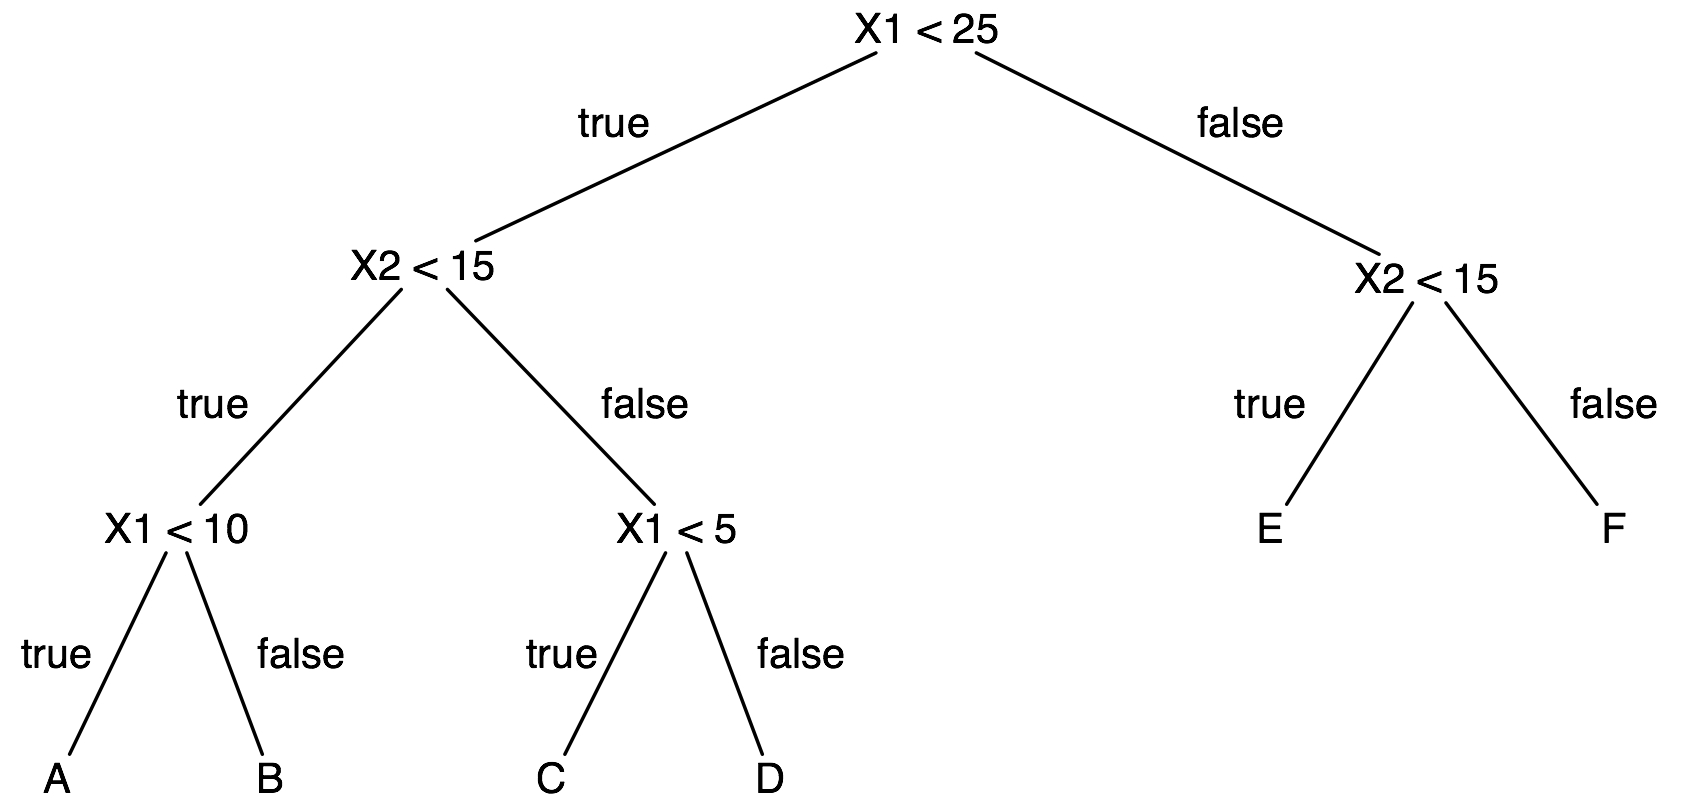
\includegraphics[scale=0.8]{dtree.jpg}
\caption{Decision tree, the base learner for random forests. From ai.cs.umbc.edu}
\label{fig:dtree}
\end{figure}

\indent Motif PSSM and GC content features lend themselves to the thresholding approach taken by decision trees. We would expect segments that are near TTS (and in the right position, e.g. the 50bp after a TTS is in the 7th segment) to have a higher PSSM score than segments that are not near TTS or in the wrong position. The classifier chooses appropriate thresholds. GC content may be another feature that differentiates TTS from non-TTS regions, or differentiates segments in each position based on some threshold.\\

\indent To train the classifier, we also need negative examples. We chose 6000 random 400bp regions in the maize genome for this. Although we did not check that none of these examples were actually near TTS, it is quite unlikely that a segment with a TTS at base pair 300 would be chosen by a random sample over the whole genome. When training the classifier, we selected an equal number of these negative examples as we had true TTS sequences. \\

\indent By evaluating cross-validation performance on the training data (negative examples and true TTS from BioMart), we selected parameters for the random forest: 300 trees, maximum depth 100, and ``entropy'' split criterion. The remaining parameters were left as default, as described in \url{http://scikit-learn.org/stable/modules/generated/sklearn.ensemble.RandomForestClassifier.html}. If the program was extended to permit more or fewer input TTS sequences, these parameters would need to be tuned. Alternatively, we could limit the overfitting of the tree by setting a minimum leaf size and/or minimum number of samples needed to add a junction at that point so that the parameters were linked directly to the dataset size.\\

{\Large\textbf{Results}}\\

\indent We applied the classifier described above to the four datasets we had downloaded from BioMart based on GO terms: salt stress, photosynthesis, water deprivation, and ribosome. Figure \ref{fig:box} shows boxplots for the accuracy, false positive rate, and false-positive rate for five trials of five-fold cross-validation. \\

\indent All classifiers achieved accuracy of 0.7-0.8, although salt stress had a bit higher performance overall. This was the largest dataset we tested in terms of number of sequences. Perhaps patterns can be more clearly characterized by the PSSM features in a larger dataset. Ribosome was the least variable in accuracy among trials (as well as FP and FN rates). In general, the false positive rate was higher than the false negative rate. To decrease the false positive rate, it may be possible to weight errors for the positive examples more than errors for the negative examples. This would be equivalent to adding copies of each positive examples and continuing to use the zero-one loss function. For this particular classification problem, false negatives would be preferred to false positives. We would rather miss putative TSS than output an overwhelming number of spurious TSS predictions.\\

\begin{sidewaysfigure}[h]
\centering
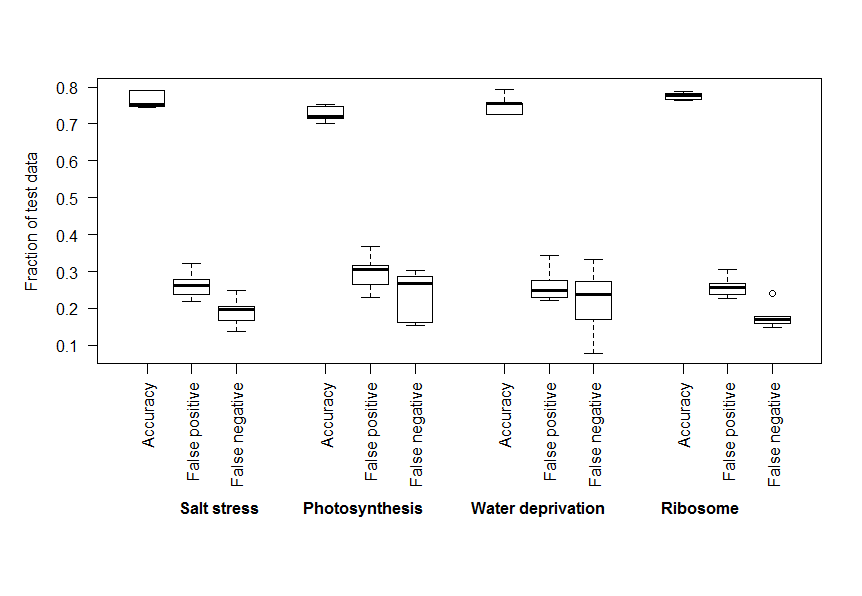
\includegraphics[scale=0.8]{Rplot.png}
\caption{Boxplot of accuracy, false positive rate, and false negative rate for four sample datasets}
\label{fig:box}
\end{sidewaysfigure}

{\Large\textbf{Scanning the genome}}\\

The prediction of new TTS in the genome is made with the Python routine\\ \texttt{finalPrediction.py}. Based on the classifier created in the previous step, 400bp regions classified as TTS in another FASTA file (can be the whole genome or a region) will be identified and outputted.\\

{\Large\textbf{Results}}\\


%TODO Results of applying all the sample dataset models to the genome.

\nocite{*}
\bibliography{references}


\end{document}
